\documentclass[12pt]{report}
\usepackage{graphicx}
\usepackage[T1]{fontenc}
\usepackage[english]{babel}
\usepackage{amsmath,amssymb}
\usepackage[a4paper, total={6in, 8.3in}]{geometry}
\usepackage{siunitx}
\usepackage{hyperref}
\usepackage{array}
\usepackage{float}

\begin{document}
\begin{titlepage}
    \centering
    \vspace*{2cm}
    \huge \textbf{Finite Element Analysis of a Harbour Crane}\\ 
    \vspace*{1cm}
    \Large \textbf{Advanced Dynamics of Mechanical Systems}\\
    \vspace{2.5cm}
    \Large
    \begin{flushright}
    Authors:\\
    \vspace{0.1cm}
    Andrea GALENDA\\Matteo FILIPPI\\Daniele FIRMANI\\Alessandro GORLA
    \end{flushright}
    \vspace{1cm}
    \vfill
    {\Large Academic Year 2023/2024\par}
\end{titlepage}

\newpage
\begin{abstract}
This report presents a Finite Element Analysis (FEA) of a harbour crane composed of steel beams. A custom FE model was developed to derive the natural frequencies and mode shapes of the structure. The analysis further explores Frequency Response Functions (FRFs) using both full FE and modal superposition approaches. Finally, the structural response is evaluated under static loads and dynamic moving loads to simulate real-world operating conditions.
\end{abstract}

\tableofcontents
\newpage

\chapter*{Theoretical Background: Cantilever Beam}
\addcontentsline{toc}{chapter}{Theoretical Background}
The fundamental objective of modal analysis is to derive the natural frequencies and mode shapes of a structure. Using a cantilever beam as a baseline analytical model, the standing wave solution is derived by applying appropriate boundary conditions (null displacement and rotation at the clamped end; moment and vertical force equilibrium at the free end). This yields an eigenvalue problem from which the structure's exact natural frequencies and continuous shape functions are computed.

Experimentally, Frequency Response Functions (FRFs) are measured for different input-output position pairs. By employing a multi-mode curve fitting method, these FRFs are approximated numerically to minimize the least-square error with the real experimental data. The modal parameters, such as natural frequencies and modal damping ratios, are extracted directly from the fitted FRFs. Finally, the mode shapes are reconstructed by evaluating the imaginary part of the FRFs at the resonant frequencies. This core theoretical foundation is directly applicable to the modal identification of much more complex physical systems.


\chapter{Finite Element Analysis of a Harbour Crane}
\section{Introduction}
This project consists of performing a Finite Element Analysis on a harbour crane made of steel beams.\\
More precisely, the aim of the first part is to derive the natural frequencies and the mode shapes of the structure.\\ 
The second one consists of employing the FE model to compute different frequency response functions for multiple input-output pairs and make a comparison with the ones obtained from the modal superimposition approach. \\
Finally the response of the structure has been computed when subjected to its own weight and to a moving load, simulating operating condition.

\section{Finite Element Model}
Firstly, a finite element (FE) model of the structure has been defined in a dedicated input file. \\
To achieve this, it has been computed the maximum element length based on the maximum frequency of interest (8 Hz), so to ensure that all elements operate in their quasi-static region within the examined bandwidth. \\
In order to have a more conservative approach, the elements employed have length between 6 m and 10 m. The obtained mesh is here reported:
\begin{figure}[H]
    \centering
    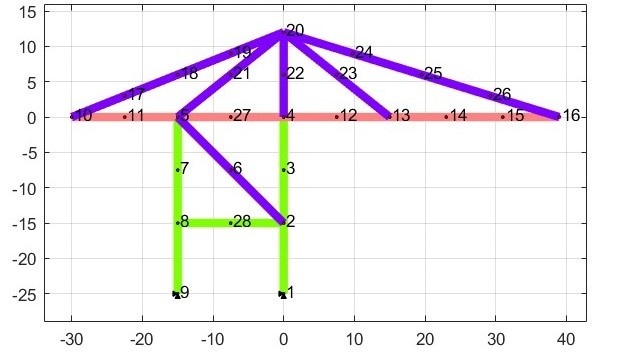
\includegraphics[scale=0.9]{figures/mesh.jpg}
    \caption{Undeformed structure and mesh}
\end{figure}

\section{Natural frequencies and mode shapes}
Once the mesh has been defined, the mass and stiffness matrices $\left[M\right]$ and $\left[K\right]$ have been assembled. This allowed to define the damping matrix $\left[C\right]$, according to the Rayleigh approach.\\
Subsequently, \(\left[M\right]\) and \(\left[K\right]\) have been partitioned into their free and constrained parts.\\
This allowed to compute the natural frequencies and the modes (up to the third one) of the structure:
\begin{table}[H]
\centering
\begin{tabular}{|c|c|c|}
\hline
\multicolumn{3}{|c|}{\textbf{Natural frequencies}} \\
\hline
1st mode & 2nd mode & 3rd mode \\ \hline
0.98 Hz          & 2.53 Hz          & 3.57 Hz          \\ \hline
\end{tabular}
\caption{Natural frequencies}
\end{table}

\noindent The resulting mode shapes are:
\begin{figure} [H]
    \centering
    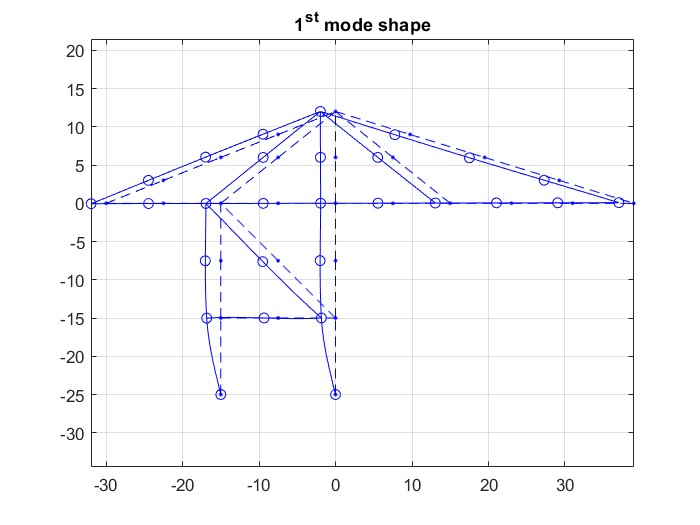
\includegraphics[scale=0.45]{figures/mode_1.jpg}
    \caption{First mode shape}
\end{figure}
\begin{figure} [H]
    \centering
    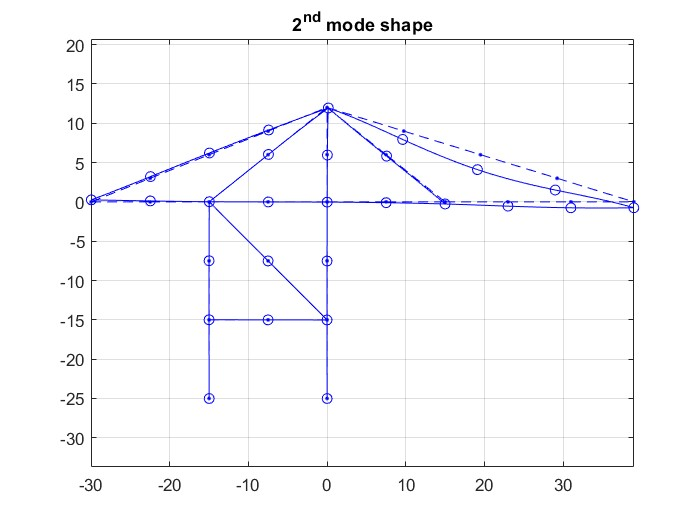
\includegraphics[scale=0.45]{figures/mode_2.jpg}
    \caption{Second mode shape}
\end{figure}
\begin{figure} [H]
    \centering
    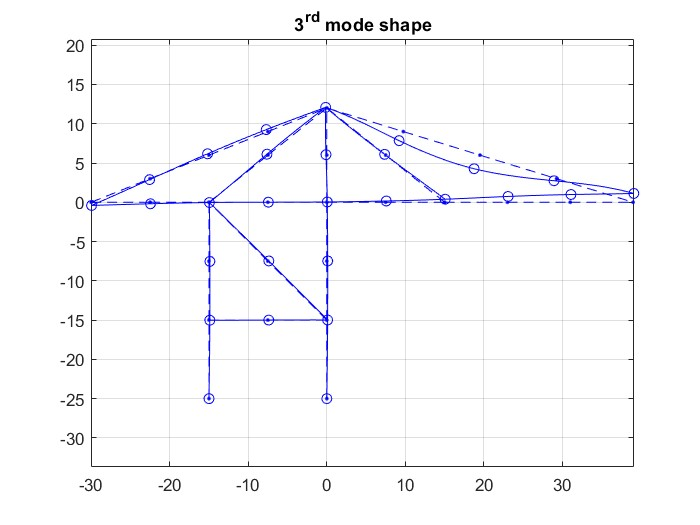
\includegraphics[scale=0.45]{figures/mode_3.jpg}
    \caption{Third mode shape}
\end{figure}

\section{Frequency Response Functions}
Then two Frequency Response Functions (FRFs) have been computed, relating a vertical input force applied in point A with two different outputs: vertical displacement in point A and horizontal displacement in point B.\\
\begin{figure}[H]
\centering

\includegraphics[scale=0.75]{Immagini report/FRFAA.jpg}
\caption{FRF: vertical force in A - vertical displacement in A}
\end{figure}
\begin{figure}[H]
\centering

\includegraphics[scale=0.75]{Immagini report/FRFAB.jpg}
\caption{FRF: vertical force in A - horizontal displacement in B}
\end{figure}
Looking at the co-located transfer function, it is possible to notice two clear resonance peaks in correspondence of the second and third eigenfrequencies, while for the first and fourth ones the function has a “flat” behaviour since point A is located near a node of the structure regarding its vertical displacement for the first and fourth mode.\\
The second FRF relates the vertical force applied in A with the horizontal displacement in B.

\section{Modal Superposition Approach}
In this section it is computed the FRF relating the vertical input force applied in node A to the horizontal displacement in point B exploiting the modal superposition approach.\\
Here is represented the FRF computed considering a unit input force:
\begin{figure} [H]
    \centering
    
\includegraphics[scale=0.75]{Immagini report/FRFAB_modfal.jpg}
    \caption{Comparison of FRF (vertical input in A, horizontal output in B) modal approach vs FE approach, considering the first 2 modes}
\end{figure}
The FRF obtained using the modal superposition catches with a good approximation the resonance peaks corresponding to the modes used to compute the modal matrix. \\

\section{Static Response and Moving Load}
The static response of the structure is obtained applying to each element a distributed load equal to its mass per unit length.
\begin{figure} [H]
    \centering
    
\includegraphics[scale=0.6]{Immagini report/static deflection.jpg}
    \caption{Static deflection due to the weight of the entire structure}
\end{figure}
The maximum static deflection is 53.6 mm and is reached in node 25.

In this section the behavior of the structure with a load moving from point D to A is analysed.\\
It starts with zero initial velocity, uniformly accelerates over the first 8 meters, keeps a constant velocity over the next 8 meters and then decelerates until reaching point A with null velocity.
\begin{figure} [H]
    \centering
    
\includegraphics[scale=0.55]{Immagini report/velocity_profile.jpg}
    \caption{Velocity profile of the load's motion}
\end{figure}
\begin{figure} [H]
    \centering
    
\includegraphics[scale=0.5]{Immagini report/Andamento.jpg}
    \caption{Time history of the vertical displacement in point A due to a moving load of 1000N}
\end{figure}
\end{document}
